\documentclass[border=10pt]{standalone}

\usepackage{tikz}
\usepackage{tikzsymbols}
\usetikzlibrary{calc,patterns,shapes.geometric}

\def\centerarc[#1](#2)(#3:#4:#5){\draw[#1] ($(#2)+({#5*cos(#3)},{#5*sin(#3)})$) arc (#3:#4:#5);}

\begin{document}
	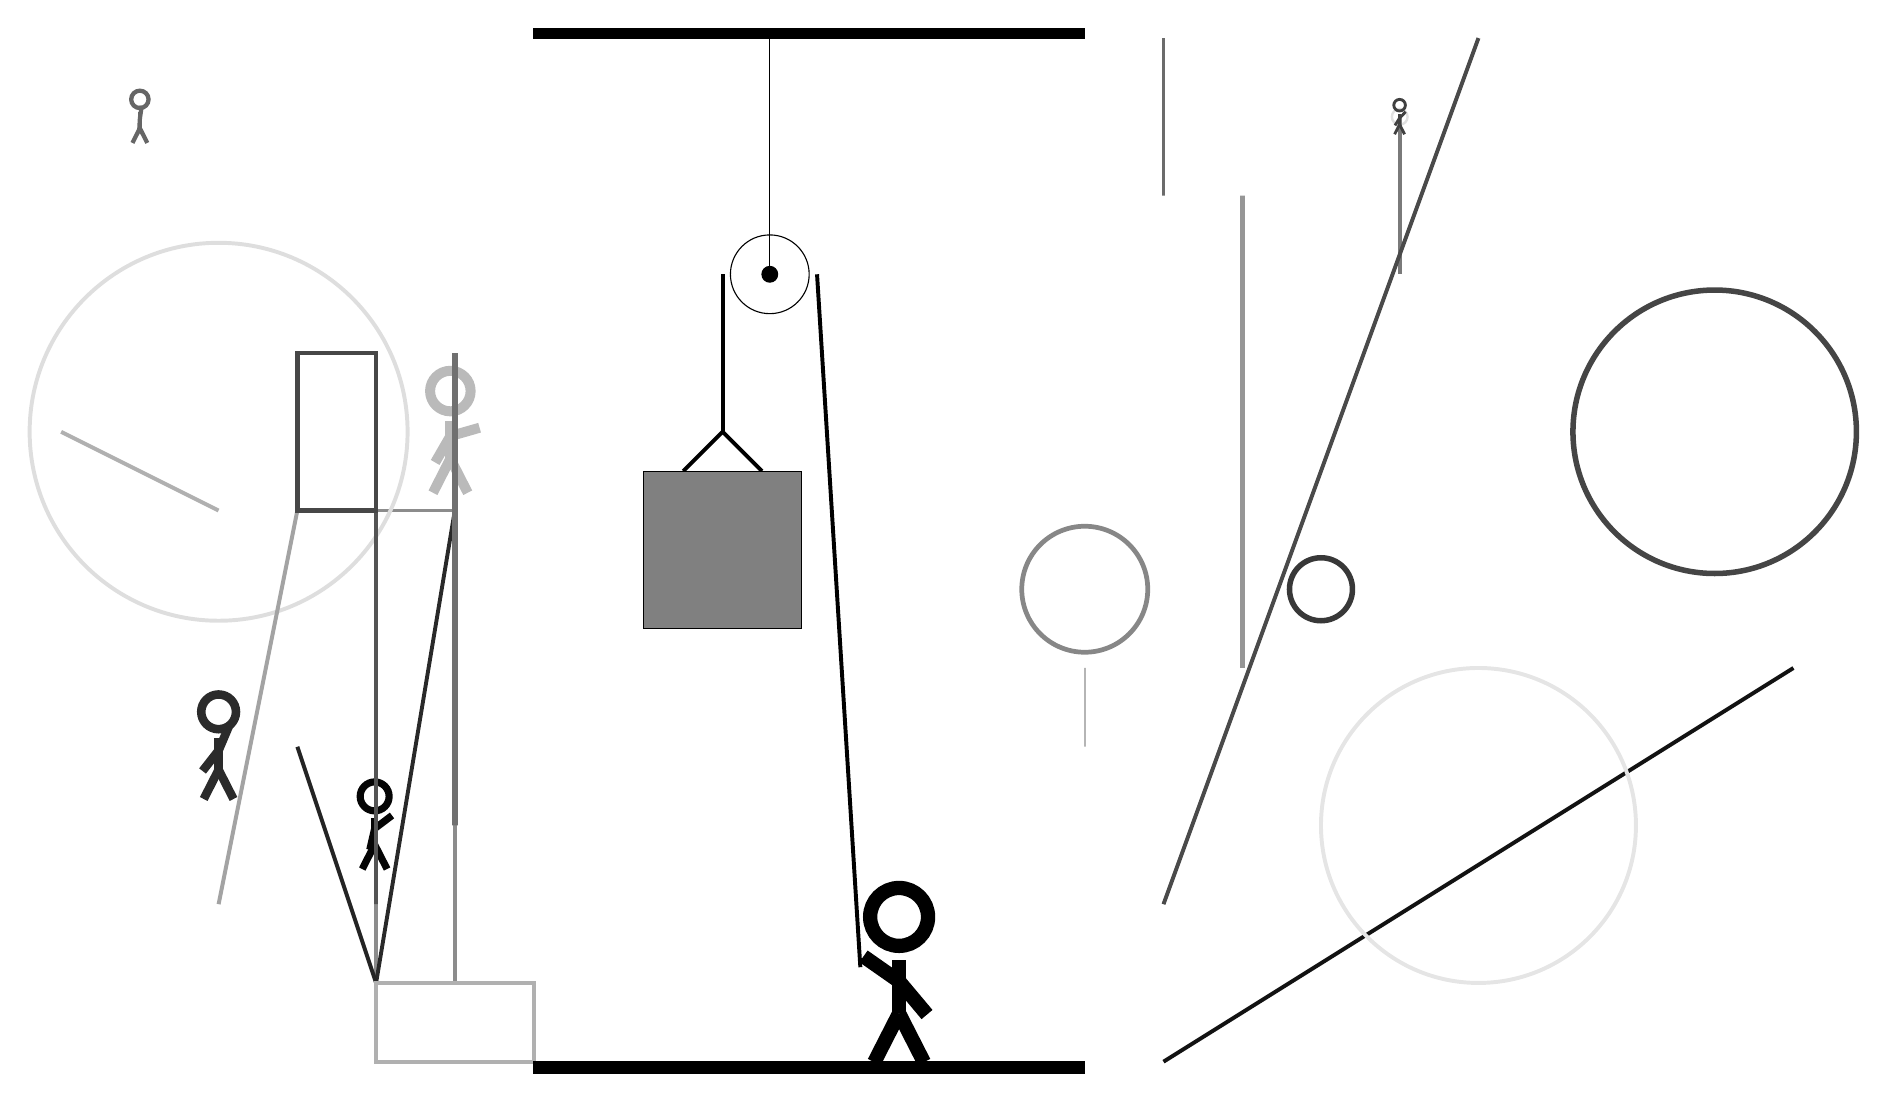
\begin{tikzpicture}
		%%%%% START %%%%%
		
		\draw[fill=black] (-2, 10) rectangle (5, 10.125);
		
		\draw (1, 7) circle (0.5);
		\draw[fill=black] (1, 7) circle (0.1);
		\draw (1, 10) -- (1, 7);
		
		\draw[line width=0.5mm] (-0.1, 4.5) -- (0.4, 5.0) -- (0.9, 4.5);
		\draw[fill=black!50] (-0.6, 4.5) rectangle (1.4, 2.5);
		
		\node[line width=0.6mm, color=black!27] at (-3, 5) {\Strichmaxerl[7][60][16]};
		
		\draw[line width=0.5mm, color=black!45] (-3, 4) rectangle (-4, -2);
		\draw[line width=0.5mm, color=black!84](-4, -2) -- (-3, 4);
		\draw[line width=0.4mm, color=black!66] (-4, 4) rectangle (-5, 6);
		\node[line width=0.4mm, color=black!98] at (-4, 0) {\Strichmaxerl[5][77][37]};
		
		\draw [line width=0.3mm, color=black!12](9, 9) circle (0.1);
		\draw [line width=0.6mm, color=black!47](5, 3) circle (0.8);
		\draw [line width=0.7mm, color=black!78](8, 3) circle (0.4);
		\draw[line width=0.5mm, color=black!86](-5, 1) -- (-4, -2);
		\draw[line width=0.2mm, color=black!29] (5, 1) rectangle (5, 2);
		\node[line width=0.4mm, color=black!60] at (-7, 9) {\Strichmaxerl[3][87][82]};
		\draw[line width=0.5mm, color=black!31](-6, 4) -- (-8, 5);
		\draw[line width=0.5mm, color=black!52](9, 9) -- (9, 7);
		
		\draw [line width=0.5mm, color=black!13](-6, 5) circle (2.4);
		\draw[line width=0.5mm, color=black!71](10, 10) -- (6, -1);
		\node[line width=0.5mm, color=black!83] at (-6, 1) {\Strichmaxerl[6][52][67]};
		\node[line width=0.5mm, color=black!75] at (9, 9) {\Strichmaxerl[2][58][46]};
		\draw[line width=0.7mm, color=black!56] (-3, 6) rectangle (-3, 0);
		\draw[line width=0.5mm, color=black!36](-6, -1) -- (-5, 4);
		
		\draw[line width=0.5mm, color=black!31] (-4, -3) rectangle (-2, -2);
		\draw[line width=0.5mm, color=black!93](6, -3) -- (14, 2);
		
		\draw [line width=0.5mm, color=black!10](10, 0) circle (2.0);
		\draw [line width=0.7mm, color=black!73](13, 5) circle (1.8);
		\draw[line width=0.5mm, color=black!67] (-4, -1) rectangle (-4, 6);
		\draw[line width=0.6mm, color=black!41] (7, 8) rectangle (7, 2);
		\draw[line width=0.5mm, color=black!58] (6, 8) rectangle (6, 10);
		\draw[line width=0.6mm, color=black!72] (-4, 6) rectangle (-5, 4);
		
		\draw[line width=0.5mm] (0.4, 7) -- (0.4, 5.0);
		\centerarc[line width=0.5mm](1, 7)(0:180:0.6);
		\draw[line width=0.5mm](1.6, 7) -- (2.15, -1.8);
		
		\node at (2.6, -1.9) {\Strichmaxerl[10][-35][-50]};
		
		\draw[fill=black] (-2, -3) rectangle (5, -3.15);
		
		%%%%% END %%%%%
	\end{tikzpicture}
\end{document}